% answers.tex —— 1959 年·全国卷 · 参考答案与详细解析片段
% 由 tools/generate_projects.py 依来源总账自 1959/1959_数学真题_试题.md + 1959/1959_数学真题_解析正文.md + 1959/1959_数学真题_答案要点.md 生成，勿手改（改源 MD 后重跑）


\gkpart{一、小题}

\begin{answer}
\gksolhead{1}{}

\textbf{题目}：

（1）已知 $\lg2=0.3010$，$\lg7=0.8451$，求 $\lg35$。

（注：$\lg$ 是以 $10$ 为底的对数的符号。）

\Needspace{4\baselineskip}
\textbf{解析}

\[
\lg35=\lg\frac{10\times7}{2}=\lg10+\lg7-\lg2=1+0.8451-0.3010=1.5441.
\]

\gkanswer{答案：$1.5441$}

\end{answer}
\begin{answer}
\gksolhead{2}{}

\textbf{题目}：

（2）化简
\[
\frac{(1-\mathrm i)^3}{1+\mathrm i}.
\]

\Needspace{4\baselineskip}
\textbf{解析}

\[
\frac{(1-\mathrm i)^3}{1+\mathrm i}
=\frac{(1-\mathrm i)^4}{(1+\mathrm i)(1-\mathrm i)}
=\frac{(1-\mathrm i)^4}{2}
=\frac{1-4\mathrm i+6\mathrm i^2-4\mathrm i^3+\mathrm i^4}{2}
=-2.
\]

\gkanswer{答案：$-2$}

\end{answer}
\begin{answer}
\gksolhead{3}{}

\textbf{题目}：

（3）解不等式：$2x^2+5x<3$。

\Needspace{4\baselineskip}
\textbf{解析}

\[
2x^2+5x<3
\iff 2x^2+5x-3<0
\iff(2x-1)(x+3)<0.
\]
两根为 $-3$、$\dfrac12$，所以
\[
-3<x<\frac12.
\]

\gkanswer{答案：$-3<x<\dfrac12$}

\end{answer}
\begin{answer}
\gksolhead{4}{}

\textbf{题目}：

（4）求 $\cos165^\circ$ 的值。

\Needspace{4\baselineskip}
\textbf{解析}

\[
\cos165^\circ=-\cos15^\circ=-\cos(45^\circ-30^\circ)
\]

\[
\cos165^\circ=-\left(\frac1{\sqrt2}\cdot\frac{\sqrt3}{2}+\frac1{\sqrt2}\cdot\frac12\right)
\]

\[
\cos165^\circ=-\frac{\sqrt6+\sqrt2}{4}
\]

\gkanswer{答案：$-\dfrac{\sqrt6+\sqrt2}{4}$}

\end{answer}
\begin{answer}
\gksolhead{5}{}

\textbf{题目}：

（5）一直圆台上底的面积为 $25\pi$ 平方厘米，下底的直径为 $20$ 厘米，母线长为 $10$ 厘米。求这直圆台的侧面积。

\Needspace{4\baselineskip}
\textbf{解析}

设圆台上、下底半径分别为 $r$、$R$，母线为 $l$。由上底面积和下底直径，
\[
\pi r^2=25\pi\Rightarrow r=5\ \mathrm{cm},
\qquad R=\frac{20}{2}=10\ \mathrm{cm},
\qquad l=10\ \mathrm{cm}.
\]
圆台侧面积为
\[
S=\pi(R+r)l=\pi(10+5)\cdot10=150\pi\ \mathrm{cm}^2.
\]

\gkanswer{答案：$150\pi\ \mathrm{cm}^2$}

\end{answer}
\begin{answer}
\gksolhead{6}{}

\textbf{题目}：

（6）有三条不在同一平面内的平行线 $a$、$b$ 和 $c$。在线 $a$ 上取一固定线段 $AB$，在线 $c$、$b$ 上各任取一点 $C$ 和 $D$。求证：不论 $C$ 和 $D$ 取在 $c$、$b$ 的什么位置上，四面体 $ABCD$ 的体积总是不变的。
\nopagebreak[4]
\begin{center}% 1959 年全国卷第 6 题：三条互不共面的平行线与四面体 ABCD。
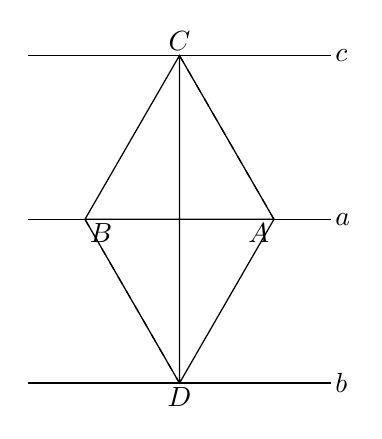
\begin{tikzpicture}[scale=0.8, line width=0.45pt,
  every node/.style={inner sep=1.5pt}]
  \coordinate (C) at (0,2.8); \coordinate (D) at (0,-2.4);
  \coordinate (B) at (-1.5,0.2); \coordinate (A) at (1.5,0.2);
  \draw (-2.4,2.8)--(2.4,2.8) node[anchor=west] {$c$};
  \draw (-2.4,0.2)--(2.4,0.2) node[anchor=west] {$a$};
  \draw (-2.4,-2.4)--(2.4,-2.4) node[anchor=west] {$b$};
  \draw (A)--(B)--(C)--cycle (A)--(D)--(B) (C)--(D);
  \draw[dashed] (C)--(A) (B)--(D);
  \draw[dashed] (C)--(D);
  \node[anchor=south] at (C) {$C$}; \node[anchor=north] at (D) {$D$};
  \node[anchor=north east] at (A) {$A$}; \node[anchor=north west] at (B) {$B$};
\end{tikzpicture}
\end{center}
\nopagebreak[4]
\Needspace{4\baselineskip}
\textbf{解析}
\nopagebreak[4]
\begin{center}% 1959 年全国卷第 6 题：三条互不共面的平行线与四面体 ABCD。
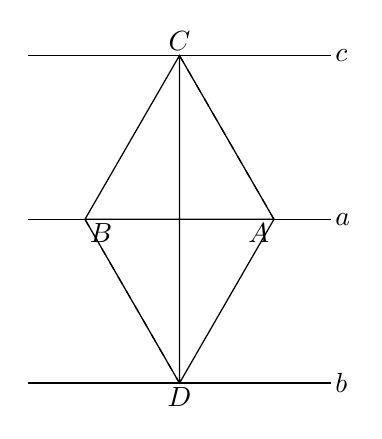
\begin{tikzpicture}[scale=0.8, line width=0.45pt,
  every node/.style={inner sep=1.5pt}]
  \coordinate (C) at (0,2.8); \coordinate (D) at (0,-2.4);
  \coordinate (B) at (-1.5,0.2); \coordinate (A) at (1.5,0.2);
  \draw (-2.4,2.8)--(2.4,2.8) node[anchor=west] {$c$};
  \draw (-2.4,0.2)--(2.4,0.2) node[anchor=west] {$a$};
  \draw (-2.4,-2.4)--(2.4,-2.4) node[anchor=west] {$b$};
  \draw (A)--(B)--(C)--cycle (A)--(D)--(B) (C)--(D);
  \draw[dashed] (C)--(A) (B)--(D);
  \draw[dashed] (C)--(D);
  \node[anchor=south] at (C) {$C$}; \node[anchor=north] at (D) {$D$};
  \node[anchor=north east] at (A) {$A$}; \node[anchor=north west] at (B) {$B$};
\end{tikzpicture}
\end{center}
\nopagebreak[4]
设平面 $\Pi$ 由平行线 $a$、$b$ 确定。由于 $AB$ 固定、$D$ 在与 $a$ 平行的直线 $b$ 上，三角形 $ABD$ 的底 $AB$ 固定，高为两平行线 $a$、$b$ 的距离，所以 $S_{\triangle ABD}$ 不变。

又因 $c\parallel a$ 且 $c$ 不在平面 $\Pi$ 内，故 $c\parallel\Pi$。点 $C$ 在 $c$ 上移动时，到平面 $\Pi$ 的距离不变。因此
\[
V_{ABCD}=\frac13S_{\triangle ABD}\,d(C,\Pi)
\]
恒定不变。

\gkanswer{答案：四面体 $ABCD$ 的体积与 $C$、$D$ 在各自平行线上所取的位置无关}

\end{answer}
\gkpart{二、大题}

\begin{answer}
\gksolhead{7}{}

\textbf{题目}：

三个数成等差数列，前两个数的和的三倍等于第三个数的二倍；如果第二个数减去 $2$（仍当作第二项），三个数就成等比数列。求原来的三个数。

\Needspace{4\baselineskip}
\textbf{解析}

设三个数为 $x-y$、$x$、$x+y$。前两个数的和的三倍等于第三个数的二倍，故
\[
3[(x-y)+x]=2(x+y)\Rightarrow4x=5y.
\]
第二个数减去 $2$ 后仍作为第二项，三数成等比数列，故
\[
(x-2)^2=(x-y)(x+y)\Rightarrow y^2-4x+4=0.
\]
代入 $x=\dfrac54y$，得
\[
y^2-5y+4=0,\qquad y=1\text{ 或 }4.
\]
分别回代，原三数为
\[
\left(\frac14,\frac54,\frac94\right)\quad\text{或}\quad(1,5,9).
\]

\gkanswer{答案：$\left(\frac14,\frac54,\frac94\right)\ \text{\text{或}}\ (1,5,9)$}

\end{answer}
\begin{answer}
\gksolhead{8}{}

\textbf{题目}：

设有 $\triangle ABC$，已知 $\angle B=60^\circ$，$AC$ 边长为 $4$，面积为 $\sqrt3$。求 $AB$ 及 $BC$ 两边之长。

\Needspace{4\baselineskip}
\textbf{解析}
\nopagebreak[4]
\begin{center}% 1959 年全国卷第 8 题：角 B=60°、AC=4 的三角形示意图。
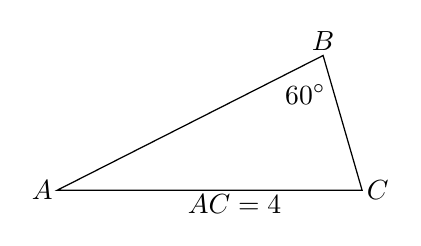
\begin{tikzpicture}[scale=0.9, line width=0.45pt,
  every node/.style={inner sep=1.5pt}]
  \coordinate (A) at (-2.5,0); \coordinate (C) at (1.8,0); \coordinate (B) at (1.25,1.9);
  \draw (A)--(B)--(C)--cycle;
  \node[anchor=east] at (A) {$A$}; \node[anchor=south] at (B) {$B$}; \node[anchor=west] at (C) {$C$};
  \node[anchor=north] at (0,0) {$AC=4$};
  \node at (1.0,1.35) {$60^\circ$};
\end{tikzpicture}
\end{center}
\nopagebreak[4]
设 $AB=x$、$BC=y$。由 $\angle B=60^\circ$、$AC=4$，余弦定理给出
\[
x^2+y^2-2xy\cos60^\circ=16,
\qquad x^2+y^2-xy=16.
\]
由面积为 $\sqrt3$，
\[
\frac12xy\sin60^\circ=\sqrt3\Rightarrow xy=4.
\]
所以 $x^2+y^2=20$，进而
\[
(x+y)^2=28,\qquad (x-y)^2=12.
\]
故
\[
x+y=2\sqrt7,\qquad x-y=\pm2\sqrt3,
\]
从而
\[
(AB,BC)=(\sqrt7+\sqrt3,\sqrt7-\sqrt3)
\]
或交换两者。

\gkanswer{答案：$(AB,BC)=(\sqrt7+\sqrt3,\sqrt7-\sqrt3)$ 或 $(\sqrt7-\sqrt3,\sqrt7+\sqrt3)$}

\end{answer}
\begin{answer}
\gksolhead{9}{}

\textbf{题目}：

$A$、$B$、$C$ 是直线 $L$ 上三点，$P$ 是这直线外一点。已知 $AB=BC=a$，$\angle APB=90^\circ$，$\angle BPC=45^\circ$。试求：

（1）$\angle PBA$ 的正弦、余弦、正切；

（2）线段 $PB$ 的长；

（3）$P$ 点到直线 $L$ 的距离。

\Needspace{4\baselineskip}
\textbf{解析}

设 $\theta=\angle PBA$、$PB=x$，且 $P$ 到直线 $L$ 的距离为 $h$。由直角三角形 $APB$，
\[
x=a\cos\theta.
\]
在三角形 $BPC$ 中由正弦定理，
\[
\frac a{\sin45^\circ}=\frac x{\sin(\theta-45^\circ)}.
\]
代入 $x=a\cos\theta$，得到 $\sin\theta=2\cos\theta$。因 $\theta$ 为锐角，
\[
\sin\theta=\frac2{\sqrt5},\qquad \cos\theta=\frac1{\sqrt5},\qquad \tan\theta=2.
\]
于是
\[
PB=x=\frac a{\sqrt5},\qquad h=x\sin\theta=\frac{2a}{5}.
\]

\gkanswer{答案：（1）$\sin\angle PBA=\dfrac2{\sqrt5}$，$\cos\angle PBA=\dfrac1{\sqrt5}$，$\tan\angle PBA=2$；（2）$PB=\dfrac a{\sqrt5}$；（3）距离为 $\dfrac{2a}{5}$}

\end{answer}
\begin{answer}
\gksolhead{10}{}

\textbf{题目}：

延长圆 $O$ 的两弦 $AB$、$CD$ 交于圆外一点 $E$，过 $E$ 点作 $DA$ 的平行线交 $CB$ 的延长线于点 $F$，自 $F$ 点作圆 $O$ 的切线 $FG$。求证 $FG=FE$。
\nopagebreak[4]
\begin{center}% 1959 年全国卷第 10 题：圆外点 E、F 与两条割线和切线 FG。
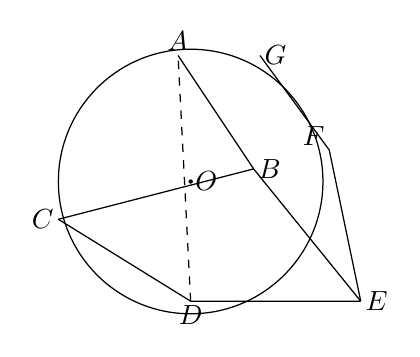
\begin{tikzpicture}[scale=0.8, line width=0.45pt,
  every node/.style={inner sep=1.5pt}]
  \coordinate (O) at (0,0); \coordinate (C) at (-2.1,-0.6); \coordinate (B) at (1.0,0.2);
  \coordinate (D) at (0.0,-1.9); \coordinate (A) at (-0.2,2.0);
  \coordinate (E) at (2.7,-1.9); \coordinate (F) at (2.2,0.5); \coordinate (G) at (1.1,2.0);
  \draw (O) circle (2.1);
  \draw (A)--(B)--(E) (C)--(D)--(E);
  \draw (E)--(F)--(G);
  \draw (C)--(B);
  \draw[dashed] (D)--(A);
  \fill (O) circle (0.035);
  \node[anchor=south] at (A) {$A$}; \node[anchor=west] at (B) {$B$};
  \node[anchor=east] at (C) {$C$}; \node[anchor=north] at (D) {$D$};
  \node[anchor=west] at (E) {$E$}; \node[anchor=south east] at (F) {$F$};
  \node[anchor=west] at (G) {$G$}; \node[anchor=west] at (O) {$O$};
\end{tikzpicture}
\end{center}
\nopagebreak[4]
\Needspace{4\baselineskip}
\textbf{解析}
\nopagebreak[4]
\begin{center}% 1959 年全国卷第 10 题：圆外点 E、F 与两条割线和切线 FG。
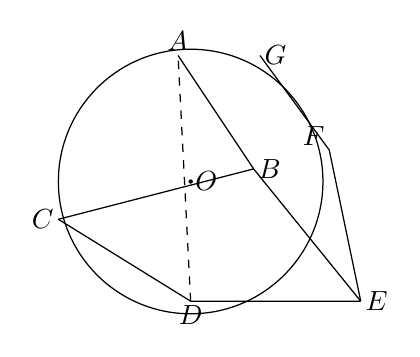
\begin{tikzpicture}[scale=0.8, line width=0.45pt,
  every node/.style={inner sep=1.5pt}]
  \coordinate (O) at (0,0); \coordinate (C) at (-2.1,-0.6); \coordinate (B) at (1.0,0.2);
  \coordinate (D) at (0.0,-1.9); \coordinate (A) at (-0.2,2.0);
  \coordinate (E) at (2.7,-1.9); \coordinate (F) at (2.2,0.5); \coordinate (G) at (1.1,2.0);
  \draw (O) circle (2.1);
  \draw (A)--(B)--(E) (C)--(D)--(E);
  \draw (E)--(F)--(G);
  \draw (C)--(B);
  \draw[dashed] (D)--(A);
  \fill (O) circle (0.035);
  \node[anchor=south] at (A) {$A$}; \node[anchor=west] at (B) {$B$};
  \node[anchor=east] at (C) {$C$}; \node[anchor=north] at (D) {$D$};
  \node[anchor=west] at (E) {$E$}; \node[anchor=south east] at (F) {$F$};
  \node[anchor=west] at (G) {$G$}; \node[anchor=west] at (O) {$O$};
\end{tikzpicture}
\end{center}
\nopagebreak[4]
由 $EF\parallel DA$，有 $\angle FEB=\angle BAD$。又圆周角所对弦相等，$\angle BAD=\angle BCD$；结合图示点列线关系，$\angle BCD=\angle FCE$，且 $\angle EFB=\angle EFC$。因此
\[
\triangle EFB\sim\triangle CFE.
\]
对应边给出
\[
\frac{FE}{FC}=\frac{FB}{FE}\Rightarrow FE^2=FB\cdot FC.
\]
另一方面，$FG$ 是切线，$FBC$ 是割线，由切割线定理
\[
FG^2=FB\cdot FC.
\]
所以 $FG^2=FE^2$，长度取正，得到 $FG=FE$。

\gkanswer{答案：$FG=FE$}

\end{answer}